\textbf{Taylor Series:} Let $f(x) = e^x$ and $g(x) = \ln(x + 1)$, and let $p_n$ and $q_n$ be the Taylor polynomials of degree $n$ for $f$ and $g$, repectively, about $x_0 = 0$.

Plot the graphs of $f$, $g$, $p_n$ and $q_n$, for some small values of $n$, and comment on your results. Discuss in particular how well $f$ and $g$ are approximated by their Taylor polynomials. Explain your observations in terms of a suitable expression for the error in the approximation.

{\color{blue}

\[
\begin{aligned}
f(x) = e^x &= 1 + x + \frac{x^2}{2!} + \frac{x^3}{3!} + \frac{x^4}{4!} + \frac{x^5}{5!} + \dots + R_n\left(x\right) \\
&= \sum_{n=0}^\infty \frac{x^n}{n!}
\end{aligned}
\]

\begin{figure}[H]
\centering
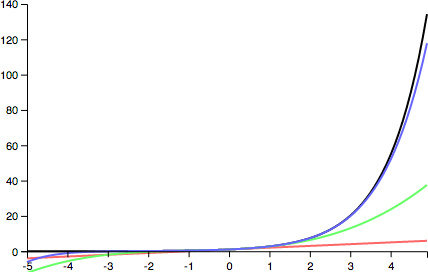
\includegraphics[scale=0.65]{taylor-series-f.png}
\caption{The Taylor polynomial of $f$ plotted for values of $n = 2$ \red{(red)}, $n = 4$ \green{(green)}, and $n = 8$ \blue{(blue)}. $f(x)$ is plotted in black. The $2$-degree Taylor polynomial is equivalent to the tangent line of $f$ at the point $x_0$. As the degree $n$ increases we have better and better approximation of the original function.}
\end{figure}

\[
\begin{aligned}
g(x) = \ln(x+1) &= x - \frac{x^2}{2} + \frac{x^3}{3} - \frac{x^4}{4} + \frac{x^5}{5} - \frac{x^6}{6} + \dots + R_n\left(x\right) \\
&= \sum_{n=1}^\infty (-1)^{n+1} \frac{x^n}{n}
\end{aligned}
\]

\begin{figure}[H]
\centering
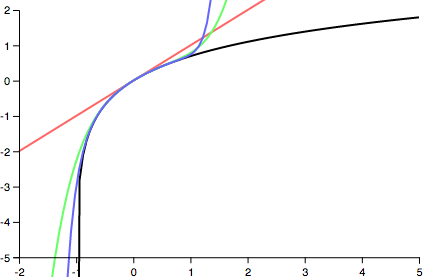
\includegraphics[scale=0.65]{taylor-series-g.png}
\caption{The Taylor polynomial of $g$ plotted for values of $n = 2$ \red{(red)}, $n = 6$ \green{(green)}, and $n = 12$ \blue{(blue)}. $g(x)$ is plotted in black. Once again when $n = 2$ we have the tangent line of $g$ at $x_0$. The Taylor polynomials for $g$ appear to be very accurate close to the center, but diverge quickly outside of this neighborhood.}
\end{figure}

The error for a Taylor polynomial can be bounded by the remainder function.
\[
|f(x) - T_n(x)| \le R_n(x) = e^x \frac{x^{n}}{n!}
\]

\[
|g(x) - T_n(x)| \le R_n(x) = \ln(x+1) (-1)^{n+1} \frac{x^{n}}{n}
\]

Where $T_n(x)$ is the Taylor polynomial for $f$ or $g$ respectively. Here as $n \to \infty$ the $|f(x) - T_n(x)| \to 0$ and $|g(x) - T_n(x)| \to 0$. For small values of $n$ the error is small around to the center point $x_0 = 0$ and grows as we move away from the center.

}
